\chapter{Using Stellar Command with OSC} \label{chap:launchosc}
There are primarily two ways to use Stellar Command. The first is as a separate process that runs on the compute. The second method is to use Stellar Command as a library that you link to directly in your program. If you intend to use Stellar Command as a library, you can skip forward to chapter~\ref{chap:libraryosc} --
\emph{\titleref{chap:libraryosc}}.


\section{Launching Stellar Command}
makeidx{standalone}
\index{osc!clientport}
\index{osc!port|}
The Stellar Command module is instantiated by executing Java  with the name of the JAR file and the required program arguments that define communication, such as the network port to send OSC messages to, and the OSC address space.  For example, to start the StellarCommand module so it sends OSC messages on UDP port 1234  using an OSC address space of \texttt{/Stellar},\footnote{In this instance, the OSC client and Stellarium are on the same computer.} one would execute the following command:\\

\begin{syntax}

	java -jar StellarCommand.jar port=1234 osc=/Stellar  \\

\end{syntax}
\bigskip
   When the server starts, it will open the first available UDP port, and notify the client of this port. For example, if the command module opened port 4567, it will send an OSC message \texttt{/Stellar/osc 4567} to the client on the localhost. 
   
\begin{syntax}

	/Stellar/osc 4567  \\

\end{syntax}
\bigskip

Allowing the command module to find its own port number removes the probability of port clashes as each client furnishes the other with a valid port number for communicating without requiring configuration in the command module. It is, however, possible to request the Stellar Command module try certain ports by adding the argument \textit{tryport} \index{osc!tryport|(} with a comma separated list of ports. For example, the argument \texttt{tryport=3333,4444,5555} will cause Stellarium to sequentially try opening the ports listed, and if these all fail, will then open the first available port.\\
   
   \begin{syntax}

   	java -jar StellarCommand.jar port=1234 osc=/Stellar  tryport=3333,4444,5555\\

   \end{syntax}
   \bigskip
   
   The OSC client would receive the following OSC message:
   \begin{syntax}
   	/Stellar/osc 3333  \\
   \end{syntax}
   \bigskip
   
The OSC client and the Stellarium server do not have to be on the same physical computer as the Stellar Command module. For example Figure~\ref{fig:RemoteStellarium}, shows three OSC clients and a Stellarium server on a LAN, and a remote Stellarium server accessible from the internet through \textit{myserver.com}. 

\begin{figure}[htbp]
	\centering
	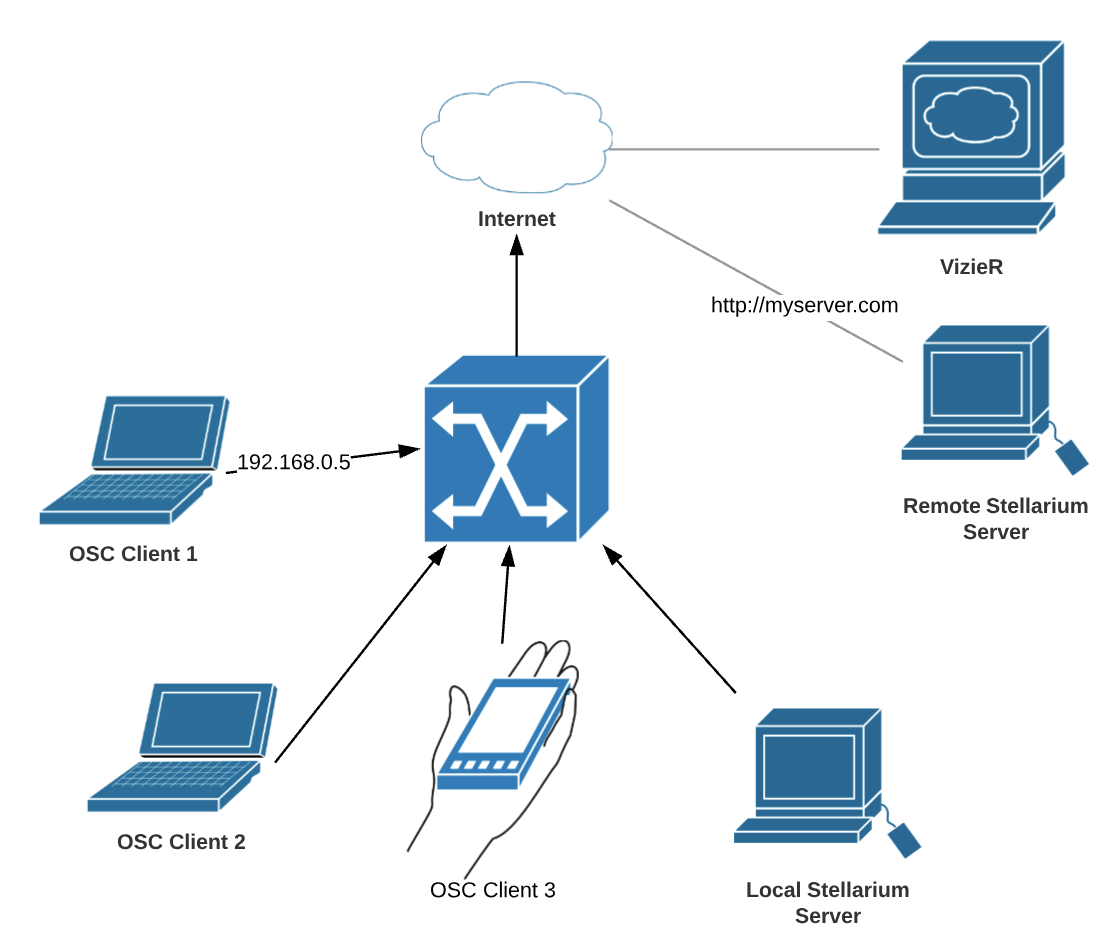
\includegraphics[width=1\columnwidth]{RemoteStellarium}
	\caption{Remote Stellarium and OSC Clients.}
	\label{fig:RemoteStellarium}
\end{figure}
\bigskip

Creating a connection between \textit{OSC Client 1} and \texttt{Remote Stellarium Server} is effected by adding adding the arguments \\\texttt{client=192.168.0.5} and \texttt{stellarium=http://myserver.com} to the command line.
This will cause the Stellar Command module to send OSC messages to ``192.168.0.5" and Stellarium commands to \textit{http://myserver.com} on HTP port 8090\footnote{The default Stellarium Remote Control port is 8090, however, this can be changed inside Stellarium. It is assumed that port forwarding when not using a local area network has been configured to send packages to the correct computer hosting Stellarium}, effectively acting as a proxy between the two.

 \begin{syntax}
	\medskip
	java -jar StellarCommand.jar port=1234 osc=/Stellar  {\char'134}\\client=192.168.0.5 stellarium=http://myserver.com\\
	\medskip
\end{syntax}
\bigskip

\section{Sending Commands to the Stellar Command Module}
You can provide instructions to Stellar Command in order to control Stellarium or to change the amount and type of data you want to receive. For example, you may want the Stellarium display to zoom in closer to a particular area of sky. You would do this by decreasing the field of view.\footnote{Section~\ref{subsec:fieldofview} --
	\emph{\titleref{subsec:fieldofview}} shows how to do this.} Likewise, you may want to reduce the amount of astronomical data you are receiving by adding a filter threshold so VizieR will only receive stars within a certain magnitude range. 

Message names are not case sensitive. For example, the messages \textit{fieldOfView} and \textit{FieldOfView} could both be used to set the field of view for Stellarium.

\subsection{poll}
Sometimes Stellar Command may already be started and configured to send and listen to the ports. You can easily find this out by sending the \textit{poll} command with no arguments, which will cause Stellarium to reply on the ports it is configured when started up.

 \begin{syntax}
	\medskip
	Stellar/poll
	\medskip
\end{syntax}

If you were sending OSC on the required port and your cleint was at the correct address, you would receive the following OSC message:
\begin{syntax}
	/Stellar/osc 3333  \\
\end{syntax}
\bigskip


\subsection{fieldOfView}\label{subsec:fieldofview}

In order to send a change in the field of view, send a message using the \textit{fieldOfView} in the namespace, followed by the field of view as a float argument. For example, to set the field of view to 60$^{\circ}$, you would send a message as follows:
 \begin{syntax}	
 	\medskip
	/Stellar/fieldOfView 60.0
	\medskip
 \end{syntax}
\bigskip

 \subsection{time}
You can set the simulation time by sending a full ISO time stamp as a string message, or by sending each Date time parameter as OSC arguments. For example, you can set the time as a string as follows:

\begin{syntax}	
	\medskip
	/Stellar/time 2019-04-18T17:51:17Z
	\medskip
\end{syntax}

If using specified time, the first three arguments will be  Year, Month and  Day as integers. The next  argument will be the hour as an integer as a 24 hour number. EG, the number 13 will signify 1pm. The next two arguments will be the minutes and seconds as integers.  The final optional argument will be the time zone as an alphabetical times zone, or if blank, the local time at the location will be used.  the same time could be set by sending the following message.
\begin{syntax}	
	\medskip
	/Stellar/time 2019 4 18 17 51 17 Z
	\medskip
\end{syntax}

Sending the following would set to midday on 18 April 2019 at the Observer location in Stellarium.

\begin{syntax}	
	\medskip
	/Stellar/time 2019 4 18 12 0 0 
	\medskip
\end{syntax}


\subsection{moveLR}
You can make the Stellarium display move left or right by sending the command \textit{moveLR} followed by a floating point number indicating how far to move. A positive value will make it appear that the viewer is turning their head to the right, while a negative number will simulate moving to the left. To move to the right, send the following command:
  \begin{syntax}	
 	\medskip
 	/Stellar/moveLR 1.0
 	\medskip
 \end{syntax}
 \bigskip

\subsection{moveUD}
You can make the Stellarium display move up or rdown by sending the command \textit{moveUD} followed by a floating point number indicating how far to move. A positive value will make it appear that the viewer is turning their head up, while a negative number will look lower. To look towards the sky, send the following command:
\begin{syntax}	
	\medskip
	/Stellar/moveUD 1.0
	\medskip
\end{syntax}
\bigskip

\subsection{azimuth}
If you want to change the azimuth that you are looking at, use \textit{azimuth} in the namespace and add the azimuth as a float argument. For example, if you wanted to turn to the east, you would send a message as follows:
 \begin{syntax}	
	\medskip
	/Stellar/azimuth 90.0
	\medskip
\end{syntax}

\subsection{altitude}
If you want to change the altitude that you are looking at, use \textit{altitude} in the namespace and add the altitude as a float argument. For example, if you wanted to look 45$^{\circ}$ up, you would send a message as follows:
\begin{syntax}	
	\medskip
	/Stellar/altitude 45.0
	\medskip
\end{syntax}

\subsection{viewAltAz}
Setting the altitude and the azimuth at the same time is so commonplace that it has been made available as a single OSC message.
If you want to change the altitude that you are looking at, use \textit{viewAltAz} in the namespace and add the altitude and then the azimuth as float arguments. The two previous calls could have been done with the single command
\begin{syntax}	
	\medskip
	/Stellar/viewAltAz 45.0 90.0
	\medskip
\end{syntax}

\subsection{viewRADec}
You can move to the RA and Dec to the centre of the sky by using  \textit{viewRADec} in the namespace and send the RA and Dec as decimal degrees. If for example, you wanted to centralise  an RA of 95.98796$^{\circ}$  and Dec. of -52.69566$^{\circ}$  (this is the star Canopus), you would send the following OSC:
 \begin{syntax}	
 	\medskip
 	/Stellar/viewRADec 95.98796 -52.69566
 	\medskip
 \end{syntax}
 
 \subsection{View Object}
 You may want to select a particular named object in the sky, such as a star, planet or moon. You can do this by using the command \textit{viewObject} followed by the object name. For example, if you wanted to centre the planet Saturn, you would send the following OSC:
 
\begin{syntax}	
 	\medskip
 	 /Stellar/viewObject Saturn
 	\medskip
 \end{syntax}
 
 \subsection{viewerObservationPoint}
 You can change the latitude, longitude, altitude and planet you are setting as your observation point by using the \textit{viewerObservationPoint} command followed by the latitude, longitude, and altitude as float arguments, and the planet as a string.  For example, to set a latitude of 32$^{\circ}$, longitude of 151$^{\circ}$, and altitude of 21m from Saturn, you would send the following command:
 
 \begin{syntax}	
 	\medskip
 	/Stellar/viewerObservationPoint 32.0 151.0 21.0 Saturn
 	\medskip
 \end{syntax}
 
 
 \subsection{showGround }
 It is possible to hide the ground, enabling you to see stars and planets through the earth by sending the \textit{showGround } command, and an integer value of zero to hide the ground or non-zero to show it. To hide the ground, you would send the following OSC message:
 
  \begin{syntax}	
 	\medskip
 	/Stellar/showGround 0
 	\medskip
 \end{syntax}

 \subsection{showAtmosphere }
It is possible to hide the atmosphere, enabling you to see stars and planets during daylight hours by sending the \textit{showAtmosphere} command, and an integer value of zero to hide the atmosphere or non-zero to show it. To hide the atmosphere, you would send the following OSC message:

\begin{syntax}	
	\medskip
	/Stellar/showAtmosphere 0
	\medskip
\end{syntax}

 \subsection{showStarLabels }
It is possible to hide the star labels  by sending the \textit{showStarLabels} command, and an integer value of zero to hide the labels or non-zero to show it. To hide the labels, you would send the following OSC message:

\begin{syntax}	
	\medskip
	/Stellar/showStarLabels 0
	\medskip
\end{syntax}

 \subsection{showConstellationart }
It is possible to show or hide the constellation art by sending the \textit{showConstellationart} command, and an integer value of zero to hide the art or non-zero to show it. To show the constellation art, you would send the following OSC message:

\begin{syntax}	
	\medskip
	/Stellar/showConstellationart 1
	\medskip
\end{syntax}

\subsection{timeRate}
It is possible to change the simulated time rate on Stellarium by sending the \textit{timeRate} command followed by the new time rate in days per second as a float. If, for example, you set the time rate to zero, time would be still and the stars would not move through the sky. If, however, you set the time rate to 0.5, the display would simulate time running at one day every two seconds. You can also make time go in reverse by setting the time rate to a negative number. To set the display to simulate a day every two seconds, you would send the following:

\begin{syntax}	
	\medskip
	/Stellar/timeRate 0.5
	\medskip
\end{syntax}

\subsection{saveTable and loadTable}
Retrieving astronomical data from VizieR can sometimes take time, depending on your internet speed and the number of stars in the field of view requested. It is possible to save the current loaded VizieR table of stars to a file so you can use it even when there is no internet. To save the table, send the command \textit{saveTable} followed by the name of the file you want it saved to. You can then use the \textit{loadTable} command later to load the data and have Stellar Command send it to you.
To save the current table to the file "Acrux.txt", send the following command:
 
 \begin{syntax}	
 	\medskip
 	/Stellar/saveTable Acrux.txt
 	\medskip
 \end{syntax}

To load this table from file and have it send the data to you, send te following command:
 \begin{syntax}	
	\medskip
	/Stellar/loadTable Acrux.txt
	\medskip
\end{syntax}

\subsection{sendStars}
It is possible to pause Stellar Command sending stars data back to the client. This may be particularly useful if you are receiving data from thousands of stars and the resources to parse decode all that data in OSC may be unnecessary. Sending the \textit{sendStars} command with a zero will cause Stellar Command to stop querying VizieR, and thus stop sending you updated astronomical data. You will still, however, receive position and field of view change messages. Sending a non-zero argument with the command will resume sending starts. To stop the data being sent, send OSC as follows:

 \begin{syntax}	
	\medskip
	/Stellar/sendStars 0
	\medskip
\end{syntax}  

\subsection{Filter}
Considering how many stars could be within a particular view, it can be beneficial to apply a filter.  For example, you may only be interested in stars with a magnitude brighter that 6. Setting a filter actually modifies the query sent to VizieR, thus reducing the amount of time to process the astronomical data.
Filtering the data is accomplished by adding the command \textit{filter}, followed by the astronomical data filed you want to filter, followed by less or greater and then using the OSC argument as the filter value.  for example, to filter the \textit{Hpmag} field so magnitudes brighter (less than) 6.5 are returned, you would send the following OSC command
   
    \begin{syntax}	
   	\medskip
   	/Stellar/filter/Hpmag/less 6.5
   	\medskip
   \end{syntax}  

You can AND filters together by sending a second command. for example, to filter stars that are between magnitudes 3 and 6, you would send the following OSC.
    \begin{syntax}	
	\medskip
	/Stellar/filter/Hpmag/less 6\\
	/Stellar/filter/Hpmag/greater 3
	\medskip
\end{syntax}  

You can filter by star colour (i.e. temperature) by filtering \textit{B-V}. For example, to filter stars with  B-V values between -1 and 1, you apply the following OSC commands:
     \begin{syntax}	
 	\medskip
 	/Stellar/filter/B-V/less 1\\
 	/Stellar/filter/B-V/greater -1
 	\medskip

You can reset the specific filter by sending a \textit{reset} command with the filter. Eg, to cleat the Hpmag filters, send the following OSC:
    \begin{syntax}	
	\medskip
	/Stellar/filter/Hpmag/reset
	\medskip
\end{syntax}  


You can reset all filters by sending the \textit{resetFilters} command:
    \begin{syntax}	
	\medskip
	/Stellar/resetFilters
	\medskip
\end{syntax}  

    
    